\documentclass[a4paper,11pt]{article}

\usepackage[margin=2.2cm]{geometry}
\usepackage{graphicx}
\usepackage{float}
\usepackage{booktabs}
\usepackage{amsmath,amssymb}
\usepackage{xcolor}
\usepackage{microtype}
\usepackage{tikz}
\usetikzlibrary{positioning,arrows.meta,backgrounds,fit,calc}
\usepackage[hidelinks]{hyperref}

\newcommand{\id}[1]{\texttt{\small #1}}
\newcommand{\vardist}{\ensuremath{d_{\mathrm{var}}}}
\newcommand{\cov}{\scriptsize}

\title{A Plug-in Family of Secret-Sharing MPC Protocols:\\
\large One $\pi$SMC Program, Many Monodromy Groups}
\author{Chenghui Weng}
\date{\today}

\begin{document}
\maketitle

\begin{abstract}
We present a family of secret-sharing multiparty computation protocols
formalised in the Rocq proof assistant on top of MathComp and infotheo. The
family is parameterised by a finite permutation group, which we call the
monodromy group, and this group drives a single shared $\pi$SMC program.
Plugging different groups into the same program leaves the program text, its
message flow, its observable effects, and its reconstructed result unchanged,
yet it changes the protocol's security and recoverability characters. We
organise the development as a small set of abstract interfaces, characterisation
records, and programs, and we instantiate it on four groups: $S_5$, the product
$S_5 \times S_5$, the wreath product $\mathbb{Z}_7 \wr S_2$, and the abelian
group $\mathbb{Z}_2 \times \mathbb{Z}_2$. A coverage analysis shows that five
abstractions are universal across all four instances, while the security and
rigidity guarantees vary through a small number of role-specific records. Every
security bound is machine-checked, and each quantitative mixing claim rests on a
single externally certified spectral inequality.
\end{abstract}

\section{Introduction}

Threshold secret sharing, introduced by Shamir~\cite{shamir1979}, lets a dealer
split a secret into shares so that any sufficiently large coalition can
reconstruct it and any smaller coalition learns nothing. In Shamir's scheme the secret is the constant term of a random
polynomial and each party holds one evaluation of it, so any $k$ shares
interpolate the secret and any fewer reveal nothing about it. We study such
protocols in a multiparty computation setting where the dealer additionally
permutes the dealt card positions by an element drawn from a fixed finite group. The secret is fixed by the starting
positions and is recovered by a reconstruction that is invariant under this
permutation, so the permutation never changes what is recovered. What it changes
is what an observer sees: it scrambles the observed positions, and the better the
permutation mixes, the closer those positions are to uniform. The permutation is
therefore a secrecy device, not a re-encoding of the secret, and secrecy of the
observables through permutation is the property the family tunes. The group that
supplies the permutation is the single tunable parameter of the whole
construction. We call it the monodromy group because, in the geometric reading
of the framework, it is the monodromy of a branched cover of the deck.

This permutation view is the abstract form of card-based secure
computation~\cite{koch2015,ruangwises2019}, where a multiparty computation is
carried out with a physical deck of cards. The foundational example is the
five-card trick of den Boer~\cite{denboer1989}: a two-party protocol that
computes the logical AND of two private bits with five cards. Each player encodes a bit as an arrangement of two cards, the players
apply a random cyclic cut to the pile, and turning the cards face up reveals the
AND and nothing more. The cyclic cut is a permutation drawn from the cyclic group
on the deck, and it is exactly the secrecy device above: it hides which input
arrangement produced the revealed pattern, while the output is read off by a
decoding that the cut leaves unchanged. Our framework keeps this structure and
lets the cut be a permutation from an arbitrary monodromy group. The cards become
the card positions, the cut becomes the group element, the computed value is
encoded in the starting positions and recovered by a permutation-invariant
reconstruction, and the strength of the secrecy is how well the group mixes the
deck. The five-card trick is then one instance of the family, recovered by taking
the group to be cyclic, and the instances studied here replace that cut by larger
groups whose mixing and recovery we analyse.

Our goal is a protocol \emph{family} in which the program is fixed and only the
plugged group varies. Concretely, the sequence of sends and receives, the value
each party observes, and the secret recovered at the end are invariant across
the family. What varies is twofold. The first varying quantity is
\emph{security}, by which we mean anonymity: how close the distribution of the
observed card positions is to the uniform distribution on the deck. The second varying
quantity is \emph{recoverability}, by which we mean both the privacy threshold
below which a coalition learns nothing and the conditions under which the dealt
secret can be reconstructed. The plug-in principle is therefore that identical
computation yields group-dependent guarantees.

The mechanism that realises this principle is a single program that is generic
over a \emph{profile}. A profile bundles the monodromy group together with a
starting layout, a security witness, and a threshold scheme. From the profile
the program reads two characters, the anonymity bound and the privacy threshold,
and it proves three guarantees, anonymity, privacy, and recovery, by consuming
the corresponding fields of the profile. Different groups give different
characters. A group whose induced random walk mixes drives the anonymity bound
to zero as the protocol runs longer, whereas a group whose walk does not mix
leaves a permanent floor. The recovery guarantee, by contrast, holds uniformly
across the family. All of these statements are proved in Rocq, so the family is
a single verified artifact rather than a paper design.

The contribution of this note is the architecture of that family and its
instantiation on four groups. Section~\ref{sec:arch} describes the abstract
artifacts and how they connect, and it opens with a coverage figure that makes
precise how few abstractions are actually needed. Section~\ref{sec:inst}
instantiates the framework on the four groups and reads off the security and
recoverability character of each.

\section{Architecture}
\label{sec:arch}

The framework factors into three kinds of artifact. \emph{Interfaces} are the
data a caller must supply, namely the monodromy group, the starting layout, and
the threshold scheme. \emph{Characterisation records} are the bundled
guarantees, namely the security witness, the covering scheme, and the rigidity
certificate. \emph{Programs} are the executable protocol, namely the profile and
the $\pi$SMC program built from it. Figure~\ref{fig:coverage} shows these
artifacts at the type level, with no instance-specific values, and for each
artifact it records which of the four instances instantiate it.

\begin{figure}[H]
\centering
\resizebox{\textwidth}{!}{%
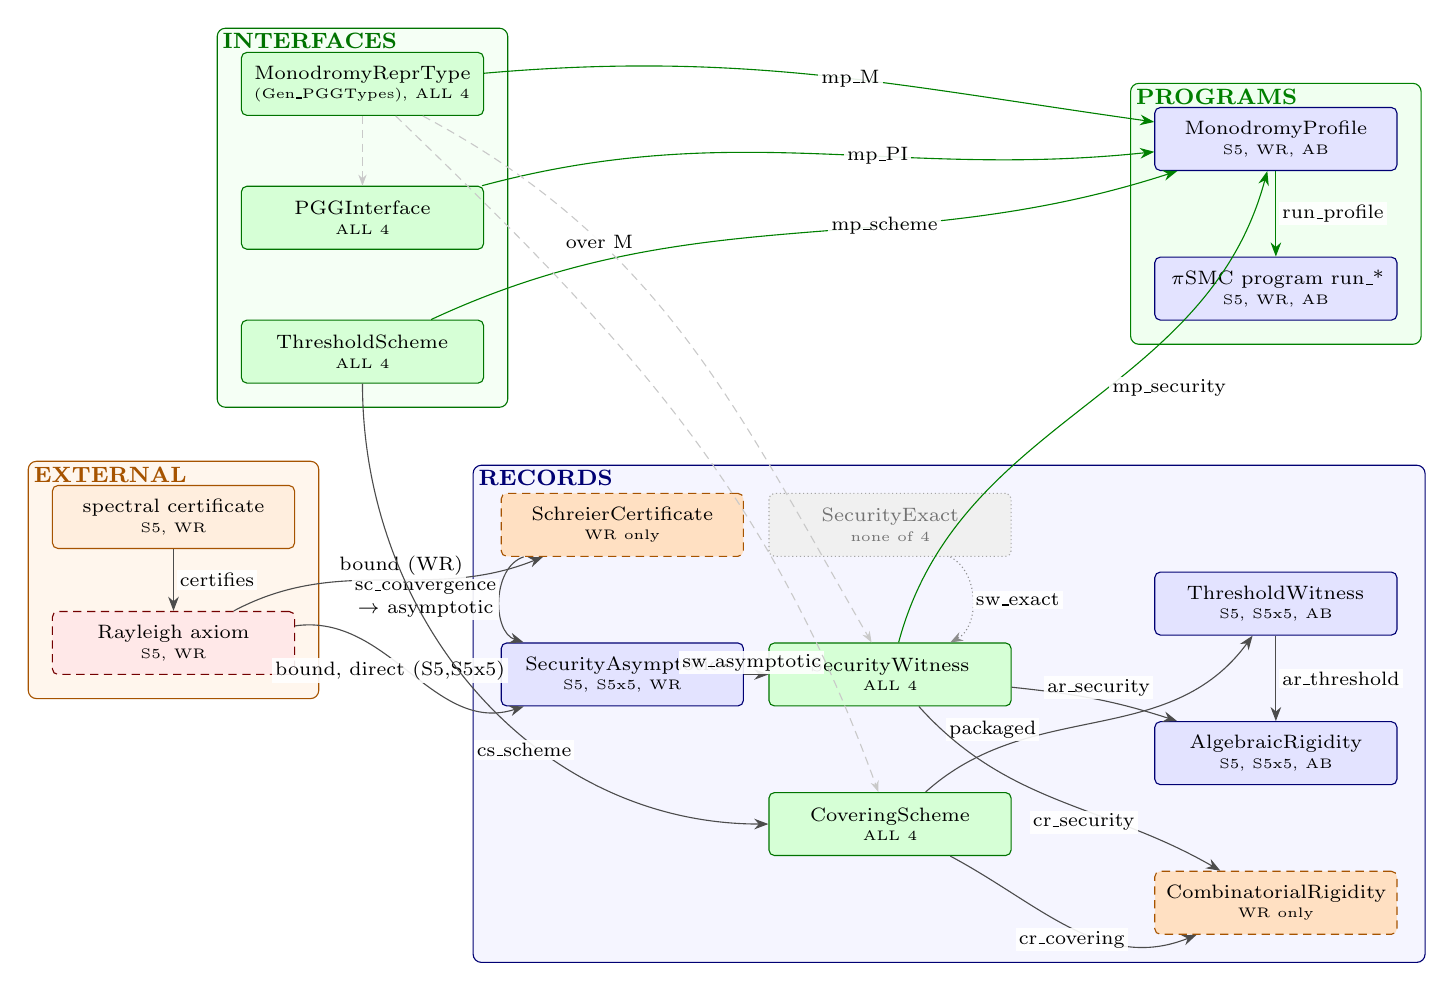
\begin{tikzpicture}[
  x=1cm, y=1cm,
  box/.style={rounded corners=2pt, draw, align=center, font=\scriptsize,
              inner sep=2.5pt, minimum height=8mm, text width=29mm},
  core/.style  ={box, fill=green!16,  draw=green!45!black},
  three/.style ={box, fill=blue!11,   draw=blue!45!black},
  only/.style  ={box, fill=orange!24, draw=orange!65!black, densely dashed},
  unused/.style={box, fill=black!6,    draw=black!35, densely dotted, text=black!55},
  axm/.style   ={box, fill=red!9,      draw=red!45!black, densely dashed},
  ext/.style   ={box, fill=orange!13,  draw=orange!65!black},
  clab/.style  ={font=\footnotesize\bfseries, inner sep=2pt, anchor=north west},
  e/.style     ={-{Stealth[length=1.8mm]}, draw=black!70, font=\scriptsize},
  eplug/.style ={-{Stealth[length=1.8mm]}, draw=green!50!black, font=\scriptsize},
  edot/.style  ={-{Stealth[length=1.6mm]}, draw=black!45, densely dotted, font=\scriptsize},
  param/.style ={-{Stealth[length=1.4mm]}, draw=gray!55, densely dashed},
  lbl/.style   ={font=\scriptsize, inner sep=1.1pt, align=center,
                 fill=white, fill opacity=0.9, text opacity=1},
]
% ---------------- INTERFACES (vertical stack, upper-left) ----------------
\node[core] (repr)   at (4.0,11.7) {MonodromyReprType\\[-1pt]{\tiny (Gen\_PGGTypes), ALL 4}};
\node[core] (pin)    at (4.0,10.0) {PGGInterface\\[-1pt]{\tiny ALL 4}};
\node[core] (scheme) at (4.0,8.3)  {ThresholdScheme\\[-1pt]{\tiny ALL 4}};
% ---------------- EXTERNAL (far left, vertical) ----------------
\node[ext]  (cert)   at (1.6,6.2)  {spectral certificate\\[-1pt]{\tiny S5, WR}};
\node[axm]  (axiom)  at (1.6,4.6)  {Rayleigh axiom\\[-1pt]{\tiny S5, WR}};
% ---------------- RECORDS (centre, 3 columns) ----------------
\node[only] (schr)   at (7.3,6.1)  {SchreierCertificate\\[-1pt]{\tiny WR only}};
\node[three](asym)   at (7.3,4.2)  {SecurityAsymptotic\\[-1pt]{\tiny S5, S5x5, WR}};
\node[unused](exact) at (10.7,6.1) {SecurityExact\\[-1pt]{\tiny none of 4}};
\node[core] (secw)   at (10.7,4.2) {SecurityWitness\\[-1pt]{\tiny ALL 4}};
\node[core] (cover)  at (10.7,2.3) {CoveringScheme\\[-1pt]{\tiny ALL 4}};
\node[three](tw)     at (15.6,5.1) {ThresholdWitness\\[-1pt]{\tiny S5, S5x5, AB}};
\node[three](alg)    at (15.6,3.2) {AlgebraicRigidity\\[-1pt]{\tiny S5, S5x5, AB}};
\node[only] (comb)   at (15.6,1.3) {CombinatorialRigidity\\[-1pt]{\tiny WR only}};
% ---------------- PROGRAMS (above RECORDS, right edge aligned to RECORDS) ----
\node[three](prof)   at (15.6,11.0) {MonodromyProfile\\[-1pt]{\tiny S5, WR, AB}};
\node[three](prog)   at (15.6,9.1)  {$\pi$SMC program run\_*\\[-1pt]{\tiny S5, WR, AB}};

% ---------------- cluster boxes (background) ----------------
\begin{scope}[on background layer]
  \node[rounded corners=3pt, draw=green!45!black, fill=green!4,
        fit=(repr)(pin)(scheme), inner sep=3mm] (ifbox) {};
  \node[rounded corners=3pt, draw=orange!65!black, fill=orange!7,
        fit=(cert)(axiom), inner sep=3mm] (extbox) {};
  \node[rounded corners=3pt, draw=blue!45!black, fill=blue!4,
        fit=(schr)(asym)(exact)(secw)(cover)(tw)(alg)(comb), inner sep=3.5mm] (recbox) {};
  \node[rounded corners=3pt, draw=green!50!black, fill=green!6,
        fit=(prof)(prog), inner sep=3mm] (progbox) {};
\end{scope}
\node[clab, text=green!45!black]  at (ifbox.north west)   {INTERFACES};
\node[clab, text=orange!65!black] at (extbox.north west)  {EXTERNAL};
\node[clab, text=blue!45!black]   at (recbox.north west)  {RECORDS};
\node[clab, text=green!50!black]  at (progbox.north west) {PROGRAMS};

% ---------------- spectral chain ----------------
\draw[e] (cert)  -- (axiom) node[lbl,midway,right=1pt]{certifies};
\draw[e] (axiom) to[out=28,in=202]  node[lbl,pos=.55,above]{bound (WR)} (schr);
\draw[e] (axiom) to[out=8,in=198]   node[lbl,pos=.4,below]{bound, direct (S5,S5x5)} (asym);
\draw[e] (schr)  to[out=-162,in=162] node[lbl,midway,left=0pt]{sc\_convergence\\$\to$ asymptotic} (asym);
\draw[e] (asym)  -- (secw)  node[lbl,pos=.32,above]{sw\_asymptotic};
\draw[edot] (exact) to[out=-28,in=28] node[lbl,midway,right=0pt]{sw\_exact} (secw);
% ---------------- recovery / scheme (routed along the bottom) ----------------
\draw[e] (scheme) to[out=-90,in=180] node[lbl,pos=.6,below=1pt]{cs\_scheme} (cover);
% ---------------- rigidity caps ----------------
\draw[e] (cover) to[out=42,in=-126] node[lbl,pos=.32,above left=-3pt]{packaged} (tw);
\draw[e] (tw)    -- (alg)  node[lbl,midway,right=1pt]{ar\_threshold};
\draw[e] (secw)  to[out=-6,in=162] node[lbl,pos=.52,above]{ar\_security} (alg);
\draw[e] (secw)  to[out=-48,in=150] node[lbl,pos=.58,below]{cr\_security} (comb);
\draw[e] (cover) to[out=-28,in=202] node[lbl,pos=.5,below]{cr\_covering} (comb);
% ---------------- program plug (green): up into PROGRAMS above RECORDS -------
\draw[eplug] (repr)   to[out=5,in=172]  node[lbl,pos=.55]{mp\_M} (prof);
\draw[eplug] (pin)    to[out=15,in=186] node[lbl,pos=.6]{mp\_PI} (prof);
\draw[eplug] (scheme) to[out=25,in=198] node[lbl,pos=.62]{mp\_scheme} (prof);
\draw[eplug] (secw)   to[out=75,in=-105] node[lbl,pos=.55,right=1pt]{mp\_security} (prof);
\draw[eplug] (prof)   -- (prog) node[lbl,midway,right=1pt]{run\_profile};
% ---------------- parameterisation (over M, dashed, faint) ----------------
\draw[param,draw=gray!42] (repr) -- (pin);
\draw[param,draw=gray!42] (repr) to[out=-28,in=120] node[lbl,pos=.3]{over M} (secw);
\draw[param,draw=gray!42] (repr) to[out=-44,in=110] (cover);
\end{tikzpicture}}
\caption{Abstract coverage of the framework across the four instances, drawn at
the type level with no instance-specific values. An external spectral
certificate justifies a Rayleigh axiom that feeds the security records; these,
with the threshold and covering records, cap off as a rigidity certificate
through the \id{ar\_*} or \id{cr\_*} fields and plug into the $\pi$SMC program
through the green \id{mp\_*} fields. The interface and record types are all
indexed by the monodromy $M$. Each node names the artifact and the instances
that instantiate it. The four instance codes are S5 $=S_5$ with 5 cards and
$|G|=120$, S5x5 $=S_5{\times}S_5$ with 10 cards and $|G|=14400$, WR
$=\mathbb{Z}_7{\wr}S_2$ with 14 cards and $|G|=98$, and AB
$=\mathbb{Z}_2{\times}\mathbb{Z}_2$ with 4 cards and $|G|=4$. The node colour is
the number of those four instances that instantiate the node: green for four,
blue for three, orange dashed for one, grey dotted for none.}
\label{fig:coverage}
\end{figure}

The figure exposes how thin the required surface is. Five abstractions are
universal, in that every instance instantiates exactly them: the monodromy
representation, the starting interface, the threshold scheme, the security
witness, and the covering scheme. Above this core each instance chooses one of
two rigidity records, and nothing uses both. The spectral sub-stack, comprising
the Rayleigh axiom and the asymptotic security record, is taken only by the
three instances whose walk mixes; the abelian instance skips it entirely. One
record, the Schreier certificate, is exercised by the wreath instance alone,
because the other two mixing instances build their asymptotic record directly.
Finally, the exact security record is present in the framework but unused by
these four instances, since it is the carrier for uniform-dealing protocols that
lie outside the present set. The remainder of this section describes each
artifact in turn.

\subsection{The $\pi$SMC Protocol}

\subsubsection{Secret-Sharing MPC}

The protocol is a threshold secret-sharing computation with parameters
$(N,T,k)$, where $N$ is the number of cards in the deck, $T$ is the number of
shares dealt, and $k$ is the privacy threshold. The dealer encodes a secret into
$T$ shares through a threshold scheme, the parties each hold one share, and a
recoverer reconstructs the secret from the collected shares. The whole protocol
is written in the $\pi$SMC calculus, a session-typed process calculus for
secure computation, so that the message discipline is checked by the session
types rather than asserted informally. The carrier of the shares is a deck of
cards, and a share is a card position in $\{0,\dots,N-1\}$.

\subsubsection{Steps}

A run proceeds in four steps. In the \emph{split} step the dealer encodes the
secret into the $T$-share tuple through the scheme's encoder. In the
\emph{compute} step the dealer applies the secrecy permutation: it hands party
$j$ the share at position $g(j)$, where $g$ is the plugged group element. In the
\emph{share} step each party forwards its received share to the recoverer. In
the \emph{recover} step the recoverer collects the $T$ shares and applies the
scheme's reconstruction, which is invariant under the permutation. The three
roles are realised by the programs \id{exchange\_dealer}, \id{exchange\_player},
and \id{exchange\_verifier}, and the dealt payload carries the plugged group's
permutation, so the group enters the protocol exactly at the compute step.

\subsubsection{Plug-in Mechanism}

The shared program is generic over a profile. The three role programs are the
same \id{exchange\_*} processes regardless of the plugged group, so the program
text, the sequence of sends and receives, and the recovered value are fixed
across the family. The only thing that changes when a different group is plugged
in is the value carried by the sends, namely the shuffled share, and through it
the distribution that an observer sees. The discriminator between a secure and
an insecure plug is therefore a property of the plugged group, for example
whether its generators commute, and not a property of the program.

\subsection{Profile}

A profile is the bundle that turns a group into a runnable protocol. It records
the monodromy representation, the starting interface, a security witness, and a
threshold scheme. A generic section consumes a profile and produces the three
role programs at the profile's interface, exposes the two characters
$\id{run\_eps}$ and $\id{run\_k}$, and proves the three guarantees. The
anonymity character $\id{run\_eps}$ is the security witness's bound, the privacy
character $\id{run\_k}$ is the scheme's threshold, the anonymity guarantee
consumes the witness's bound field, the privacy guarantee consumes the scheme's
sub-threshold indistinguishability, and the recovery guarantee consumes the
scheme's correctness. Because all three guarantees are projections of profile
fields, a profile is exactly the evidence needed to run the program securely.

\subsection{Security}

The security witness is the always-present record of anonymity. Its mandatory
field is a bound stating that, for every starting card, the variation distance
between the observed endpoint distribution and the uniform distribution is at
most a stated $\varepsilon$. On top of this bound the witness carries two
optional slots, an exact slot and an asymptotic slot, which record stronger
information when it is available.

\subsubsection{Exact}

The exact slot carries a closed-form equality for $\varepsilon$, that is, a proof
that the variation distance equals a stated value rather than merely being
bounded by it. This slot is appropriate when the shuffle is dealt uniformly or
when the endpoint distribution can be counted exactly. None of the four
instances of this note use the exact slot, since their security comes from a
random walk rather than from uniform dealing; the slot is the carrier used by
the uniform-dealing protocols that lie outside the present set.

\subsubsection{Asymptotic}

The asymptotic slot carries a geometric convergence certificate. It states that
the variation distance at protocol length $L$ is at most
$\varepsilon_\infty + \sqrt{N}\,(1-\gamma)^{L}$, where $\gamma$ is a spectral
gap and $\varepsilon_\infty$ is an additive floor. When the induced walk is
irreducible the floor is zero and the bound decays to zero, so anonymity becomes
perfect in the limit. When the walk is reducible the floor is positive and
records the gap between mixing on an orbit and mixing on the whole deck. The
asymptotic slot is what distinguishes a mixing plug from a floored one.

\subsection{Threshold}

The threshold scheme records the secret-sharing structure independently of the
group. It fixes the number of shares $T$ and the privacy threshold $k$, and it
supplies an encoder, a reconstructor, a correctness proof that reconstruction
inverts encoding, and a privacy proof that any coalition of fewer than $k$
shares cannot distinguish two secrets. The difference $T-k$ is a
privacy-and-reveal gap rather than a dropout budget, because reconstruction
consumes the full share tuple. The scheme is the recoverability counterpart of
the security witness: the witness governs what an observer learns about the
shuffle, and the scheme governs what a coalition learns about the secret.

\subsection{Rigidity}

A rigidity record bundles security and recoverability into a single certificate
for an instance. It always carries a security witness and a covering scheme, and
it adds a structural statement about the group. The framework provides two
rigidity records, and each instance uses exactly one.

\subsubsection{Algebraic}

The algebraic rigidity record pairs a security witness with a threshold witness,
where the threshold witness packages a covering scheme together with an
obligation that, if the covering has genus zero, then the group order is at most
the curve's automorphism bound. This record suits instances whose certification
is organised around a covering of a fixed genus, including the cases where the
genus-zero obligation is discharged vacuously because the covering has positive
genus.

\subsubsection{Combinatorial}

The combinatorial rigidity record pairs a security witness with a covering scheme
and adds two explicit fields: that the covering genus is positive and that the
group order strictly exceeds the curve bound. This record states the
large-group-with-positive-gap configuration directly, and it is the positive
dual of a no-go theorem that forbids the same configuration for any genus-zero
realisation of the relevant representation. It suits an instance that realises
recoverability through a positive-genus covering rather than a vacuously
discharged genus-zero one.

\subsection{Spectral}

The spectral layer supplies the asymptotic security record for the mixing
instances. The induced random walk on the deck has a transition matrix $Q$, and
its mixing rate is governed by the second-largest eigenvalue modulus. The
asymptotic bound reduces to a Rayleigh inequality $\langle v, Q^2 v\rangle \le
\alpha^2 \langle v, v\rangle$ for mean-zero vectors $v$, where $\alpha$ bounds
that eigenvalue. This inequality is certified externally by an exact-rational
sum-of-squares factorisation and is imported into the development as a single
axiom. The remaining ingredient is symmetry of $Q$, which the framework obtains
in one of two ways: from involutive generators, when each generator squares to
the identity, or from an inverse-closed generating multiset, when the generators
are not involutions. The Schreier certificate record packages the spectral gap
with the resulting convergence bound and yields the asymptotic security record
generically.

\section{Instances}
\label{sec:inst}

We instantiate the framework on four groups. Each instance fixes a monodromy
group, hence a deck and a walk, and then selects a rigidity record and a security
character. Table~\ref{tab:inst} summarises the four, and the subsections read off
each one.

\begin{table}[h]
\centering
\small
\begin{tabular}{@{}lllrll@{}}
\toprule
instance & group & deck & $|G|$ & rigidity & security character \\
\midrule
$S_5$ & $S_5$ & 5 & 120 & algebraic & asymptotic, floor $0$ \\
$S_5\times S_5$ & $S_5\times S_5$ & 10 & 14400 & algebraic & asymptotic, floor $1$ \\
$\mathbb{Z}_7\wr S_2$ & wreath & 14 & 98 & combinatorial & asymptotic, floor $0$ \\
$\mathbb{Z}_2\times\mathbb{Z}_2$ & abelian & 4 & 4 & algebraic & floored, no asymptotic \\
\bottomrule
\end{tabular}
\caption{The four instances. Floor $0$ means anonymity becomes perfect in the
limit; floor $1$ is the un-halved variation-distance floor of a reducible walk;
the abelian instance has a permanent floor and carries no asymptotic record.}
\label{tab:inst}
\end{table}

\subsection{$S_5$: adjacent transpositions}

The first instance takes $S_5$ generated by the four adjacent transpositions of
the path on five vertices, acting on a deck of five cards. The induced walk is
the path-graph walk, which is irreducible, so the asymptotic security record has
floor zero. Its spectral gap is $1 - 181/200 = 19/200$, certified by the
instance's own sum-of-squares script. The instance uses the algebraic rigidity
record, with a positive-genus covering whose genus-zero obligation is discharged
vacuously, and it builds its asymptotic record directly rather than through the
Schreier certificate. It also plugs into the shared program as one of the three
profiles, where its privacy threshold is read off the scheme.

\subsection{$S_5 \times S_5$: two piles}

The second instance takes the direct product $S_5 \times S_5$, with one $S_5$
acting on each of two piles of five cards, on a deck of ten cards. Because the
two piles never exchange cards, the walk is reducible: a card that starts in one
pile stays there forever. The walk therefore mixes only within an orbit, and its
asymptotic security record has a positive floor, equal to one in the un-halved
variation-distance convention. The instance reuses the $S_5$ Rayleigh
certificate rather than carrying its own, since each component walk is an $S_5$
walk, and its recovery side is a two-component covering by two disjoint copies of
the underlying curve. It uses the algebraic rigidity record and does not plug
into the shared program.

\subsection{$\mathbb{Z}_7 \wr S_2$: the wreath}

The third instance takes the wreath product $\mathbb{Z}_7 \wr S_2$ of order
ninety-eight, acting on a deck of fourteen cards arranged as two piles of seven.
Its two within-pile generators are seven-cycles and its third generator is the
pile swap. The seven-cycles are not involutions, and $\mathbb{Z}_7$ has odd
order, so the group cannot be generated by involutions at all and the bare
transition matrix is not symmetric. The instance recovers symmetry by adjoining
the inverse generators, which leaves the group unchanged but makes the
generating multiset inverse-closed, and it proves symmetry of the transition
matrix from that inverse-closure. The walk is then irreducible, so the
asymptotic security record has floor zero, with spectral gap $1 - 17/20 = 3/20$,
wider than the $S_5$ gap. This instance is the only one that exercises the
Schreier certificate record, and it uses the combinatorial rigidity record,
whose positive-genus and order-inequality fields realise the configuration that
the no-go theorem forbids for a genus-zero realisation. It also plugs into the
shared program.

\subsection{$\mathbb{Z}_2 \times \mathbb{Z}_2$: the abelian baseline}

The fourth instance takes the abelian group $\mathbb{Z}_2 \times \mathbb{Z}_2$
generated by two commuting disjoint transpositions, acting on a deck of four
cards. The two generators stabilise a two-card block setwise, so a card that
starts in the block never leaves it, and the endpoint distribution keeps zero
probability on a card outside the block for every protocol length. The variation
distance is therefore bounded below by a fixed positive constant, independent of
length, so the walk does not mix and the security witness carries no asymptotic
record. The instance is the insecure baseline of the family: it certifies its
recoverability through a genus-zero covering built from Reed-Solomon codes, which
is exactly Shamir's secret-sharing scheme~\cite{shamir1979}, together with the
algebraic rigidity
record, and it plugs into the same shared program as the mixing instances, where
it exhibits the permanent floor that the mixing plugs escape.

\bibliographystyle{plain}
\bibliography{20260605T063044Z-pgg_protocol_family}

\end{document}
